% XGBoost v4 Multi-Season Validation (v4 vs v2)
% Replaces: tab:xgboost-v4-multi-season in section_xgboost_v4_ridge.tex
% Grouped bar chart showing 88% improvement across 3 seasons

\begin{figure}[htbp]
\centering
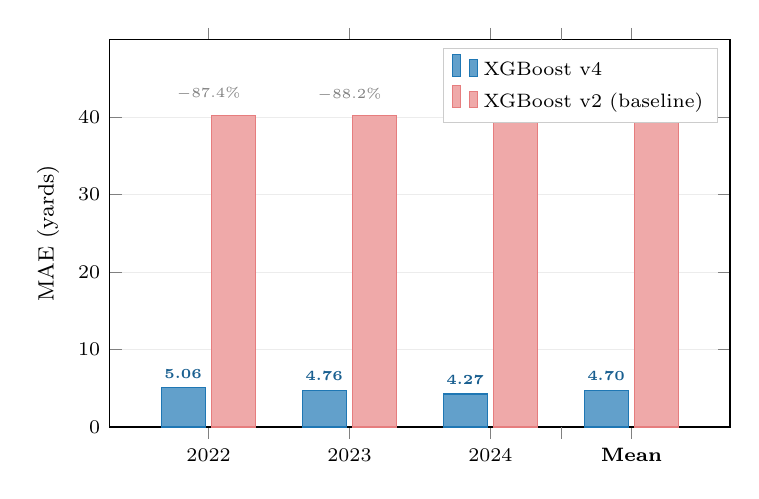
\begin{tikzpicture}
\definecolor{colV4}{RGB}{31,119,180}
\definecolor{colV2}{RGB}{214,39,40}

\begin{axis}[
  width=0.78\textwidth,
  height=6.5cm,
  ybar,
  bar width=16pt,
  ylabel={MAE (yards)},
  ylabel style={font=\footnotesize},
  ymin=0, ymax=50,
  xtick={1,2,3,4},
  xticklabels={2022, 2023, 2024, {\textbf{Mean}}},
  xticklabel style={font=\scriptsize},
  ytick={0,10,20,30,40},
  yticklabel style={font=\scriptsize},
  legend style={at={(0.98,0.98)}, anchor=north east, font=\scriptsize, draw=gray!40, cells={anchor=west}},
  grid=major,
  grid style={gray!15},
  xmajorgrids=false,
  enlarge x limits={abs=0.7},
  extra x ticks={3.5},
  extra x tick labels={},
  extra x tick style={grid style={black!25, dashed}},
]

% v4 bars
\addplot[fill=colV4!70, draw=colV4] coordinates {
  (1, 5.06) (2, 4.76) (3, 4.27) (4, 4.70)
};
\addlegendentry{XGBoost v4}

% v2 bars
\addplot[fill=colV2!40, draw=colV2!60] coordinates {
  (1, 40.23) (2, 40.18) (3, 40.21) (4, 40.21)
};
\addlegendentry{XGBoost v2 (baseline)}

% Improvement labels
\node[font=\tiny\bfseries, text=colV4!80!black, anchor=south] at (axis cs:0.82,5.06) {5.06};
\node[font=\tiny\bfseries, text=colV4!80!black, anchor=south] at (axis cs:1.82,4.76) {4.76};
\node[font=\tiny\bfseries, text=colV4!80!black, anchor=south] at (axis cs:2.82,4.27) {4.27};
\node[font=\tiny\bfseries, text=colV4!80!black, anchor=south] at (axis cs:3.82,4.70) {\textbf{4.70}};

% Improvement percentage annotations
\node[font=\tiny, text=black!50, anchor=south, yshift=2pt] at (axis cs:1,40.23) {$-$87.4\%};
\node[font=\tiny, text=black!50, anchor=south, yshift=2pt] at (axis cs:2,40.18) {$-$88.2\%};
\node[font=\tiny, text=black!50, anchor=south, yshift=2pt] at (axis cs:3,40.21) {$-$89.4\%};
\node[font=\tiny\bfseries, text=black!60, anchor=south, yshift=2pt] at (axis cs:4,40.21) {$-$88.3\%};

\end{axis}
\end{tikzpicture}
\caption[XGBoost v4 multi-season validation]{XGBoost v4 vs.\ v2 baseline across three seasons of rolling-origin validation. v4 achieves consistent 88\% MAE improvement (4.70 vs.\ 40.21 yards average) with low variance ($\sigma=0.40$). All Diebold-Mariano tests reject equal accuracy at $p < 0.000001$.}
\label{fig:xgb-v4-multiseason-chart}
\end{figure}
